\begin{center}
\begin{figure}[ht]
\begin{center}
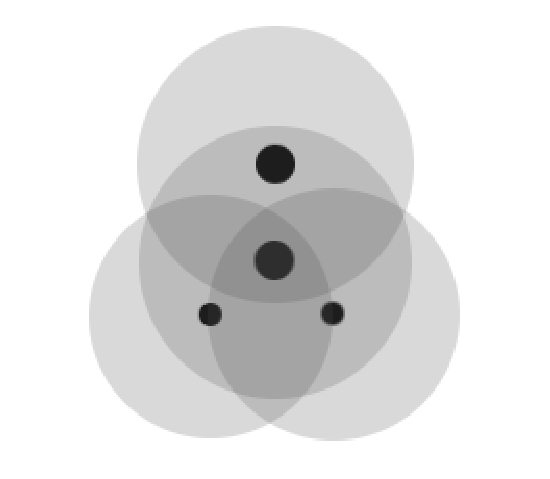
\includegraphics[width=5cm]{03_nevpt/images/rydberg1.eps}
\includegraphics[width=5cm]{03_nevpt/images/rydberg2.eps}
\end{center}
\caption{\footnotesize Two possible schemes to define an augmented basis set
for the description of diffuse Rydberg orbitals: adding diffuse functions on
the single atoms (left side of the picture) or adding diffuse functions
supported by a single dummy atom with no charge. In this thesis, the
development of the Rydberg orbitals followed the second approach.}
\label{fig:rydberg}
\end{figure}
\end{center}
